% EN48 c08 | 原书 p.110 下部–113（PDF 119–122） | 第 4 章 §4.4
% 块边界：p.110 上半的 §4.3 收尾归 c07；本块从 §4.4 正文起（\subsection 标题已在骨架中）。
\subsection{$H^0(\mathrm{FS}(Y,v_0))$：定义与选择的无关性}

% ===== 原书 p.110 =====

现在进入深谷--Seidel 范畴的定义。所考虑的拉格朗日都是线性的，因此带有提升，可用斜率给出 Maslov 分次；它们还带有 Spin 结构。

\transnote{「用斜率给出 Maslov 分次」是本文一切计数的前提：拉格朗日在紧集外投影成射线，射线的角度就给出一个整数分次。若没有这个分次，$\hom$ 只是 $\Z/2$-分次的，式~\eqref{c8:eq-hom} 里的 $0$ 次交点也就无从谈起。}

\begin{definition}\label{c8:def-fs}
深谷--Seidel 范畴 $FS(Y,v_0)$ 的定义如下。这里用范畴局部化的方法，取代 [Sei08] 的 Hamilton 扰动方法：
\begin{itemize}[leftmargin=1.6em,itemsep=0.25em]
\item 对象：$FS(Y,v_0)$ 中的拉格朗日，也就是全空间中的拉格朗日，允许非紧。
      拉格朗日 $L_i$ 的取法：在 $v_0$ 的底空间中取 $-1$ 上方的 $\ell_i$，沿 U 形曲线绕过零上方的奇异纤维，作平行移动（图~\ref{c8:fig-Li}）。
      具体地说，在原点周围某个紧集之外，这些拉格朗日必须投影为平面中的射线，并且是纤维化的——即纤维中拉格朗日的平行移动。
\item 态射：定义一个有向范畴
\begin{equation}\label{c8:eq-hom}
\hom(K,L)=
\begin{cases}
CF(K,L), & K>L,\\
\C\cdot 1, & K=L,\\
0, & \text{其他},
\end{cases}
\end{equation}
      其中序 $>$ 指：在紧集之外，$K$ 的所有射线都在 $L$ 的所有射线之上。
      若 $K=L$，则把其中一份的射线推高，使其位于另一份的射线之上（图~\ref{c8:fig-Li}），单位 $e_L$ 就是以这些拉格朗日为边界条件的盘的计数。
      这一推的过程给出 $L^\eps$。随后在这些 $e_L$ 处局部化，也就是把它们设为同构。
      回忆一下，形式地反转态射要取 roofs 的等价类
      \[
      K\leftarrow K^\eps\rightarrow L ;
      \]
      当 $K<L$ 时，这就是箭头 $K\to L$ 的定义：先把 $K$ 推到 $K^\eps>L$，使 roof 的第一个箭头是拟同构，而 $K^\eps\to L$ 按上面的方式定义。
\item 微分（$\mu^1$）、复合（$\mu^2$）与高阶 $\mu^k$ 分别数二边形、三角形与 $(k+1)$ 边形。
      这些映射是原书 4.3.5 意义下的类截面映射，带有这些 $L_i$ 给出的通常拉格朗日边界条件，并对某个正则 $J$ 全纯（其存在性见上文）。
      这些模空间可用上一节的理论来数。
\item 注意，这里把 $T_z$ 排除在所考虑的子范畴的对象之外——它是 $t_z$ 绕底空间中一个圆作平行移动所得——以免因盘起泡而在定义 $\hom(T_z,T_z)$ 时动用 bounding cochains。
\end{itemize}
\end{definition}

\transnote{数边形的对应关系容易数错：$\mu^k$ 有 $k$ 个输入、$1$ 个输出，故对应 $(k+1)$ 边形。$\mu^1$ 是二边形（条带）、$\mu^2$ 是三角形、$\mu^3$ 是四边形。这里的「边」按边界分支数算，不按顶点数算。}

\transnote{把 $T_z$ 排除在外，是本文避免 bounding cochains 的办法。$T_z$ 在底空间中是一个圆上的平行移动，围绕它的盘会起泡；一旦起泡，$\hom(T_z,T_z)$ 的计数就不能只数模空间，还得先选 bounding cochain 作「增广」。本文的子范畴不需要这些对象，故直接略去。}

% ===== 原书 p.111 =====

\begin{figure}[tbp]
\centering
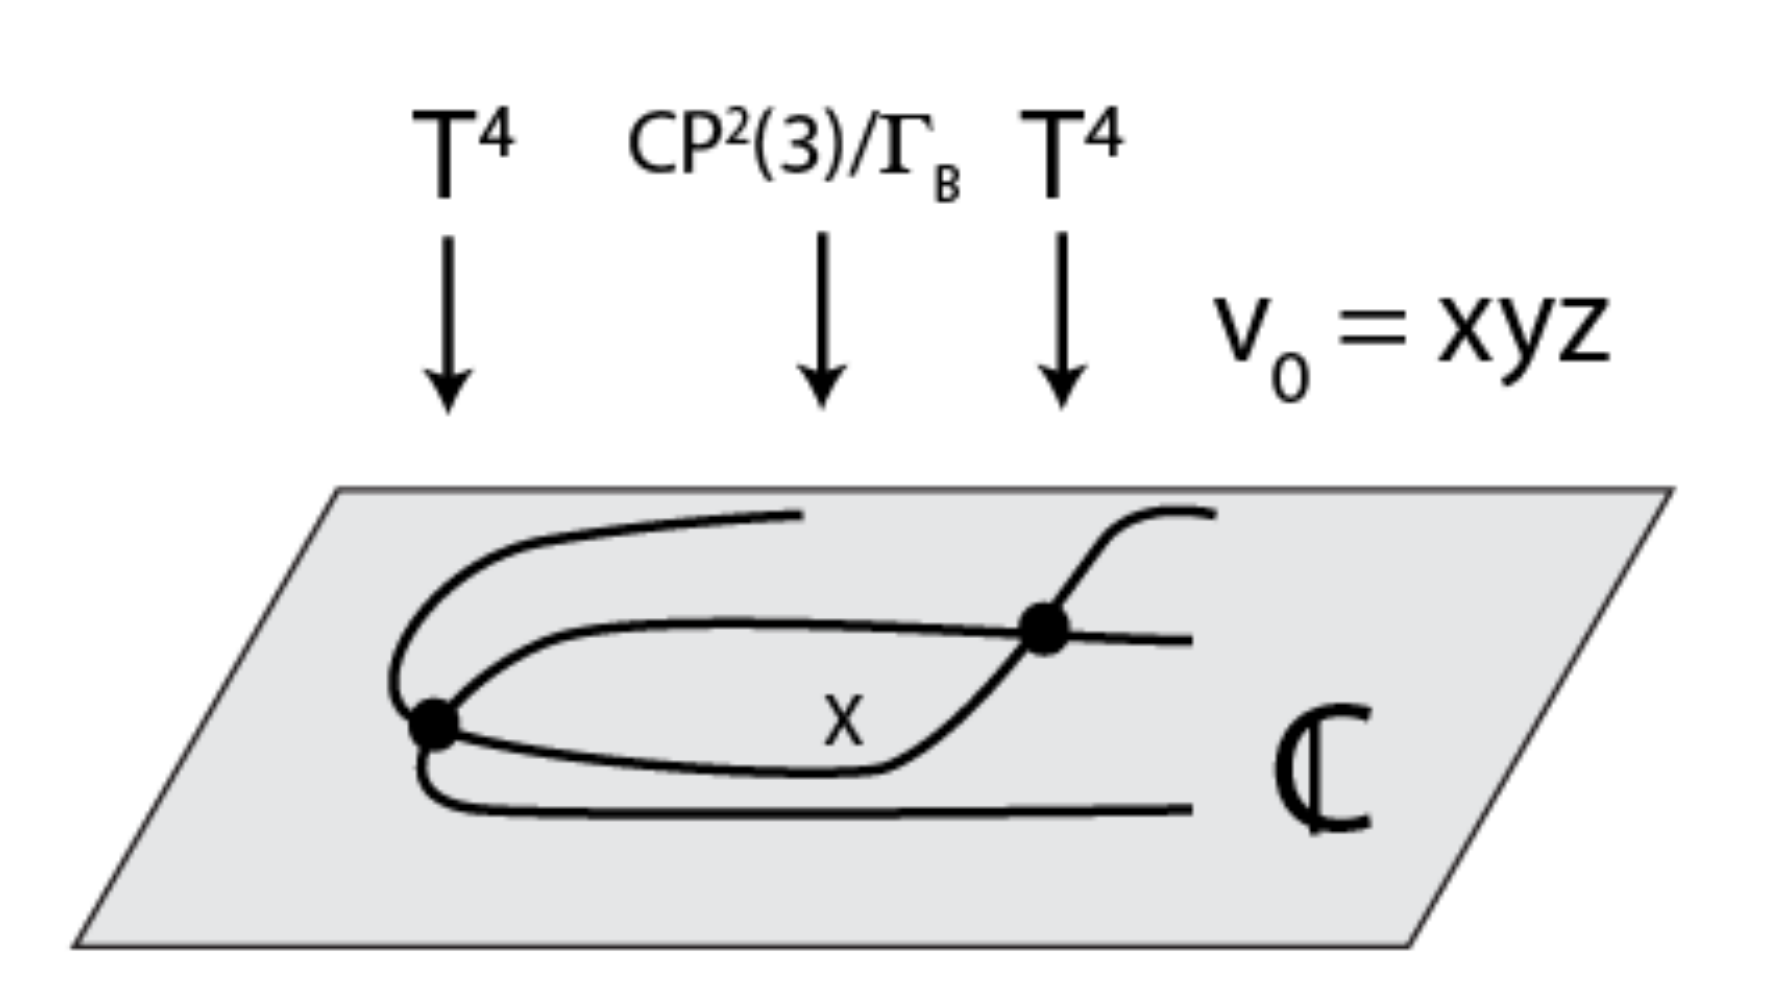
\includegraphics[width=0.64\textwidth]{figures/fig_4_5.png}
\caption{$L_i$：把 $\ell_i$ 沿 $v_0$ 底空间中的 U 形曲线平行移动（原书 p.111）}
\label{c8:fig-Li}
\end{figure}

\transnote{对象的「纤维化」要求是本文与 [Sei08] 的关键差别。这里只允许沿 U 形曲线平行移动所得的拉格朗日，它们在紧集之外投影成射线；正因为如此，才能像式~\eqref{c8:eq-hom} 那样按射线的上下位置定义一个序，而不必先做 Hamilton 扰动。}

\begin{lemma}\label{c8:lem-hom-position}
局部化范畴中 hom 的落位正确；论证见 Abouzaid--Seidel、Ganatra 的笔记与 Abouzaid--Auroux。
\end{lemma}

\begin{lemma}\label{c8:lem-roof}
roofs 的复合仍是 roof。
\end{lemma}

\begin{proof}
参见 M. Jeffs 的硕士论文。
\end{proof}

\transnote{读 roof 时注意箭头的方向与谁是拟同构。$K<L$ 时，先沿推射线把 $K$ 抬成 $K^\eps$，使它高于 $L$；此时按式~\eqref{c8:eq-hom}，$K^\eps\to L$ 才有定义（因为 $K^\eps>L$），而 $K\to K^\eps$ 是拟同构。原文说「形式地反转态射」，指的就是把本不存在的 $K\to L$ 用这条 roof 来表达。}

% ===== 原书 p.112 =====

\begin{remark}[单位]\label{c8:rem-units}
在 Floer 理论中 $\mathrm{HF}(V,V)\cong H(V;\KK/2)$。
$2$-环面（$T^4$ 纤维中「高度为零」的部分）的上同调环：$0$ 次与 $2$ 次为 $\Z$，$1$ 次由 Künneth 公式为 $\Z\oplus\Z$。
上链层面的生成元个数确实相同。
\end{remark}

\transnote{$\KK/2$ 不是把系数域除以 $2$，而是半整数分次：单位所在的次数可以落在 $\frac12\Z$ 里。对照下一句「上链层面生成元个数相同」，作者是在说：$V$ 的上同调按 $\Z$ 分次算出的生成元，与按 $\frac12\Z$ 分次算出的相同。}

\begin{definition}\label{c8:def-donaldson-fukaya}
Donaldson--Fukaya 范畴：对态射链复形取上同调即得。
它是拓扑量子场论的一个例子，即从流形到向量空间、把配边映到向量空间同态的函子。
\end{definition}

\begin{lemma}\label{c8:lem-J-indep}
设 $J_1$ 与 $J_2$ 是两个正则近复结构，则它们给出拟等价的 Fukaya $A_\infty$-范畴。
\end{lemma}

\begin{proof}
见 Seidel §8 与 §(10c)。
\end{proof}

\transnote{「拟等价」与「拟同构」要分清：两个范畴之间的 $A_\infty$ 函子若每个态射复形上都诱导拟同构，就称拟等价；两个对象之间的态射若在同调上诱导同构，才叫拟同构。本条的结论是在范畴层面说的，故用「拟等价」。}

\begin{remark}\label{c8:rem-indep-discussion}
[Sei08] 的 (10a) 与 (10b) 讨论了这件事，但超出我们的需要。[Sei08] 的 (10c) 含 Donaldson--Fukaya 范畴同构的论证。

我们可以构造一个 $A_\infty$ 函子（如前所述，它就是恒等），见 [Sei08] 开头；于是不必考虑同伦。
一般情形下这不对，因为 $\mu^2$ 可能跳；但这里不会，因为所有交点都在 $0$ 次。
我们有线性的连续映射，高阶的都是恒等。

FOOO 与 Floer 的经典做法是构造同伦。见 [FOOO09a, p 244]：同伦的代数背景在第 4.2 节；引入虚拟基本链之后，定理用于 Fukaya 范畴情形，见该书 Corollary 4.6.3 或他们 2000 年预印本的 Theorem 15.19。

Seidel 把 $J$ 的各选择所对应的所有 Fukaya 范畴打包成一个「总」Fukaya 范畴，从而把这一套升级到 $A_\infty$ 情形。
他证明每个 $\cF(Y)_i$ 都全忠实嵌入总范畴，并借助 Salamon--Zehnder 对实际范畴的工作，在上同调上诱导同构。
于是所有 $\cF(Y)_i$ 都拟同构于同一个对象，从而彼此拟同构，证明完成。

注意，[FOOO09a, p 244] 讨论了 $J$-不变性。代数同伦不变性在第 4.2 节讨论，主定理在第 4.6 节。
两者之间，他们把几何基本链搭成第 4.2 节代数理论的一个应用。

一般地，用单个 PDE 在两个 $J$ 之间插值的连续映射论证，给出每个选择下 Floer 群的同构；Seidel 在 [Sei08, §(10c)] 讨论了如何把它升级到 $A_\infty$-范畴。
\end{remark}

\transnote{这里说「不必考虑同伦」，前提是所有交点都在 $0$ 次，故 $\mu^2$ 不会跳。一般情形下 $\mu^2$ 是可能跳的，那时必须像 FOOO 与 Floer 那样显式构造同伦；原文特意点出这一点，读者不要把它当成普遍结论。}

% ===== 原书 p.113 =====

\begin{corollary}\label{c8:cor-well-defined}
此范畴与正则数据的选择无关，故良定义。
特别地，足够小的不同 $T$ 值给出拟同构的 Fukaya 范畴——定义复结构时 $\Gamma_B$ 有可商的正纯全纯群作用。
\end{corollary}

\begin{proof}
对正则 $J$ 的不变性已如上。纤维中 Hamilton 扰动下的不变性，文献中已有。
这就完成了「良定义的 Fukaya 范畴」的证明。
\end{proof}

\begin{remark}\label{c8:rem-family}
技术上，我们会有一个 $T$ 上一族 Fukaya 范畴之间的镜像对应，故复结构 $J_T$ 涉及缩放标准 $J$，并缩放 A 侧的辛形式。
要证不变性，得看近复结构空间中的一条连通路径，即缩放这个 $T$ 所得的路径。
\end{remark}

\transnote{最后这条注把视野放大到 $T$ 上的整族范畴。$T$ 是复结构的参数，缩放 $T$ 同时缩放两侧：$B$ 侧的复结构、$A$ 侧的辛形式。原文说「看近复结构空间中的连通路径」，就是要在缩放过程中逐点比较范畴，而不是孤立地比两个 $T$ 值。}

\transnote{本块收束第 4 章。原书把「不依赖选择」这件事分成两层：正则 $J$ 的选择，与纤维中 Hamilton 扰动的选择。前者靠上一节的 Sard--Smale 与模空间理论，后者在文献里已有；两者合起来才得到良定义的 $H^0(FS(Y,v_0))$。}
